%-----------------------------------------------------------------------------------%
\section{Introduction\label{sec:intro2dm}}
%-----------------------------------------------------------------------------------%

I'll attempt to explain the dark matter problem at an entry level with the following thought experiment.
Let's say you're the teacher for an elementary school classroom.
You take them on a field trip to your local science museum and among exhibits is one for mass and weight.
The exhibit has a gigantic scale, and you come up with a fun problem for your classroom.

You say to your class, "What is the total weight of the classroom?
Give your best estimation to me in 30 minutes, and then we'll check on the scale.
If your guess is within 10\% of the right answer, we will stop for ice cream on the way back"

The students are ecstactic to hear this, and they get to work.
The solution is some variation of the following strategy.
The students should give each other their weight or best guess if they don't know.
Then, all they have to do is add each students' weight and get a grand total for the class.
The measurement on the giant scale should show the true weight of the class.
When comparing the measured weight, multiply the observation by 1.1 and 0.9 in order to get the +/- 10\% tolerance respectively.

Two of your students, Sandra and Mario, return to you with a solution.

They say, "We weren't sure of everyone's weight.
We used 65 lbs for the people we didn't know and added everyone who does know.
There are 30 of us, and we got 2,000 lbs!
That's a ton!"

You estimated 1,900 lbs assuming the average weight of a student in your class was 60 lbs.
So you're pleased with Sandra's and Mario's answer.
You instruct your students to all gather on the giant scale and read off the weight together.
To all of your surprise, the scale reads \textit{10,000 lbs}!
10,000 is significantly more than a 10\% error from 2,000.
In fact, it is approximately 5 times more massive than either your or your students' estimates.
You think to yourself and conclude there must be something wrong with the scale.
You ask an employee to check the scale and verify it is calibrated well.
They confirm that the scale is in working order.
You weigh a couple of students individually to test that the scale is well calibrated.
Sandra weighs 59 lbs, and Mario weighs 62 lbs, typical weights for their age.
You then weigh each student individually and see that their weights individually do not deviate greatly from 60 lbs.
So, where does all the extra weight come from?

This thought experiment serves as an analogy to the Dark Matter problem.
The important substitution to make however is to replace the students with stars and classroom with a galaxy, say the Milky Way.
Individually the mass of stars is well measured and defined with the Sun as our nearest test case.
However, when we set out to measure the mass of a collection of stars as large as galaxies, our well motivated estimation is wildly incorrect.
There simply is not way to account for this discrepancy except without some unseen, or dark, contribution to mass and matter in galaxies.
I set out in my thesis to narrow the possibilities of what this Dark Matter could be.

This chapter is organized like the following\dots
\todo{Text should look like ... Chaper x has blah blah blah.}

%-----------------------------------------------------------------------------------%
\section{Dark Matter Basics\label{sec:basicDM}}
%-----------------------------------------------------------------------------------%

Presently, the most compelling Dark Matter (DM) model is $\Lambda$ \textbf{C}old \textbf{D}ark \textbf{M}atter, or \lcdm.
I present the evidence supporting \lcdm~in \ref{sec:evidence4dm}, yet discuss the conclusions of the \lcdm~model here.
According to \lcdm~fit to observations on the Cosmic Microwave Background (CMB), DM is 26.8\% of the universe's current energy budget
Baryonic matter, stuff like atoms, gas, and stars, contributes to 4.9\% of the universe's current energy budget \cite{Greene:cosmology_dm,Young:cosmology_dm,Bertone:particleDM}.

% A note on the above, the number is usually quoted as some \Omega_{f} h^_2. In order to get the percentages yourself, you need to actually multiply h which is the hubble expansion rate.

DM is dark; it doesn't interact readily with light at any wavelength.
DM also doesn't interact noticably with the other standard model forces (Strong and Weak) at a rate that is readily observed \cite{Bertone:particleDM}.
DM is cold, which is to say that the average velocity of DM is below relativisic speeds \cite{Greene:cosmology_dm}.
'Hot' DM would not likely manifest the dense structures we observe like galaxies, and instead would produce much more diffuse galaxies than what is observed \cite{Bertone:particleDM,Greene:cosmology_dm}.
DM is old; it played a critical role in the formation of the universe and the structures within it \cite{Greene:cosmology_dm,Young:cosmology_dm}.

Observations of DM has so far been only gravitational.
The parameter space available to what DM could be therefore is very broad.
Searches for DM are summarized by supposing a hypothesis that has not yet been ruled out, and performing measurements to test them.
When the observations yield a null result, the parameter space is further constrained.
I present some approaches for DM searches in \cref{sec:dm_search}.

%-----------------------------------------------------------------------------------%
\section{Evidence for Dark Matter}\label{sec:evidence4dm}
%-----------------------------------------------------------------------------------%

Dark Matter (DM) has been a looming problem in physics for almost 100 years.
Anomolies have been observed in galactic dynamics as early as 1933 when Fritz Zwicky noticed unusually large velocity dispersions in the Coma cluster.
Zwicky's measurement was the first recorded to use the Virial theorem to measure the mass fraction of visible and invisible matter in celestial bodies~\cite{Hooper:DMHistory}.
From Zwicky in \cite{Zwicky:1933}, "\textit{If this would be confirmed, we would get the surprising result that dark matter is present in much greater amount than luminous matter.}"
Zwicky's and other's observation did not instigate a crisis in astrophysics because the measurements did not entirely conflict with their understanding of galaxies \cite{Hooper:DMHistory}.
In 1978, Rubin, Ford, and Norbert measured rotation curves for ten spiral galaxies \cite{Rubin:1978}.
Rubin et. al.'s 1978 publication presented a major challenge to the conventional understanding of galaxies that could no longer be accreditted to measurement uncertainties.
Evidence has been mounting ever since for this exotic form of matter.
The following subsections sample some of the compelling evidence supporting DM.

%$$$$$$$$$$$$$$$$$$$$$$$$$$$$$$$$$$$$$$$$$$$$$$$$$$$$$$$$$$$$$$$$$$$$$$$$$$$$$$$$$$$%
\subsection{First Clues: Stellar Velocities\label{sec:ev4dm_stars}}
%$$$$$$$$$$$$$$$$$$$$$$$$$$$$$$$$$$$$$$$$$$$$$$$$$$$$$$$$$$$$$$$$$$$$$$$$$$$$$$$$$$$%

Zwicky's, and later Rubin's, measurement of the stellar velocities were built upon the Virial theorem, shown as \virialtheorem
Where \textit{T} is the kinetic energy and \textit{V} is the potential energy in a self-gravitating system.
The potential was defined as the classical Netwon's law of gravity from stars and gas contained in the observed galaxies \newtongravity
Zwicky et. al. measured just the velocities of stars apparent in optical wavelengths \cite{Zwicky:1933}.
Rubin et. al. added by measuring the velocity of the hydrogen gas via the 21 cm emmission line of Hydrogen \cite{Rubin:1978}.
The velocities of the stars and gas are used to infer the total mass of galaxies and galaxy clusters via \cref{eq:virialtheorem}.
An inferred mass is also made from the luminosity of the selected sources.
The two inferences are compared to each other as a luminosity to mass ratio and typically yields \cite{Greene:cosmology_dm}\masslightratio
$M_{\sun}$ and $L_{\sun}$ referring to stellar mass and stellar luminosity respectively.
These ratios clearly indicate a discrepancy in apparent light and mass from stars and gas and their velocities.

Rubin et.al. \cite{Rubin:1978} demonstrated that the discrepancy was unlikely to be an under-estimation of the mass of the stars and gas.
The inferred 'dark' mass was up to 5 times more than the luminous mass.
This dark mass also needed to extend well beyond the extent of the luminous matter.

\begin{figure}[h]
    \centering{
    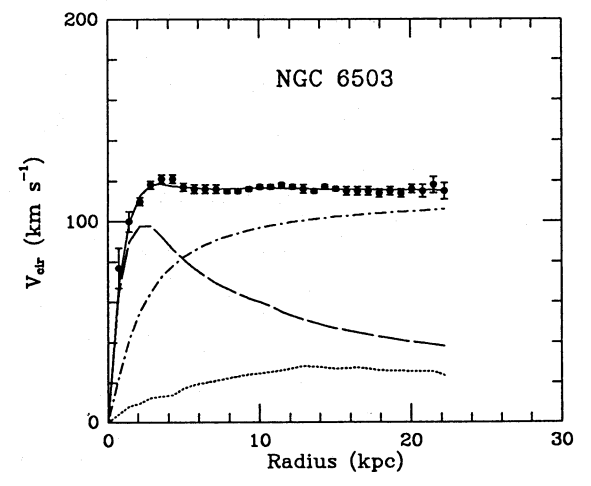
\includegraphics[scale=0.7]{figures/NGC6503_rotcurve.png}
    \caption{Rotation curve fit to NGC 6503 from \cite{Begeman:rot_curves}. Dashed line is the contribution from visible matter. Dotted curves are from gas. Dash-dot curves are from dark matter (DM). Solid line is the composite contribution from all matter and DM sources. Data are indicated with bold dots with error bars. Data agree strongly with matter + DM composite prediction}
    \label{fig:gal_rot_curve}
    }
\end{figure}

\cref{fig:gal_rot_curve}: features one of many observations made on the stellar velocities within galaxies.
The measured roation curves mostly feature a flattening of velocities at higher radius which is not expected if the gravity was only coming from gas and luminous matter.
The extension of the flat velocity region also indicates that the DM is distributed far from the center of the galaxy.
Modern velocity measurements include significantly larger objects, galactic clusters, and smaller objects, dwarf galaxies.
Yet, measurements along this regime are leveraging the virial theorem with Newtonian potential energies.
We know Netwonian gravity is not a comprehensive description of gravity.
New observational techniques have been developed since 1978, and those are discussed in the following sections.

%$$$$$$$$$$$$$$$$$$$$$$$$$$$$$$$$$$$$$$$$$$$$$$$$$$$$$$$$$$$$$$$$$$$$$$$$$$$$$$$$$$$%
\subsection{Evidence for Dark Matter: Micro-lensing\label{sec:ev4dm_lens}}
%$$$$$$$$$$$$$$$$$$$$$$$$$$$$$$$$$$$$$$$$$$$$$$$$$$$$$$$$$$$$$$$$$$$$$$$$$$$$$$$$$$$%

Modern evidence for dark matter comes from new avenues beyond stellar velocities.
Gravitational micro-lensing from DM is a new channel from general relativity.
The Cosmic Microwave Background shows that the universe had DM in it from a very early stage.
Computational resources have expanded greatly in recent decades enabling universe models that again support the need for DM in the evolution of the universe.

General relativity predicts abberations in light caused by massive objects.
In recent decades we have been able to measure the lensing effects from compact objects and DM haloes.
\cref{fig:grav_lensing_explained} shows how different compact bodies change the final image of a far away galaxy resulting from gravitational lensing.
Gravitational lensing developed our understanding of dark matter in two important ways.

\begin{figure}[h!]
    \centering{
        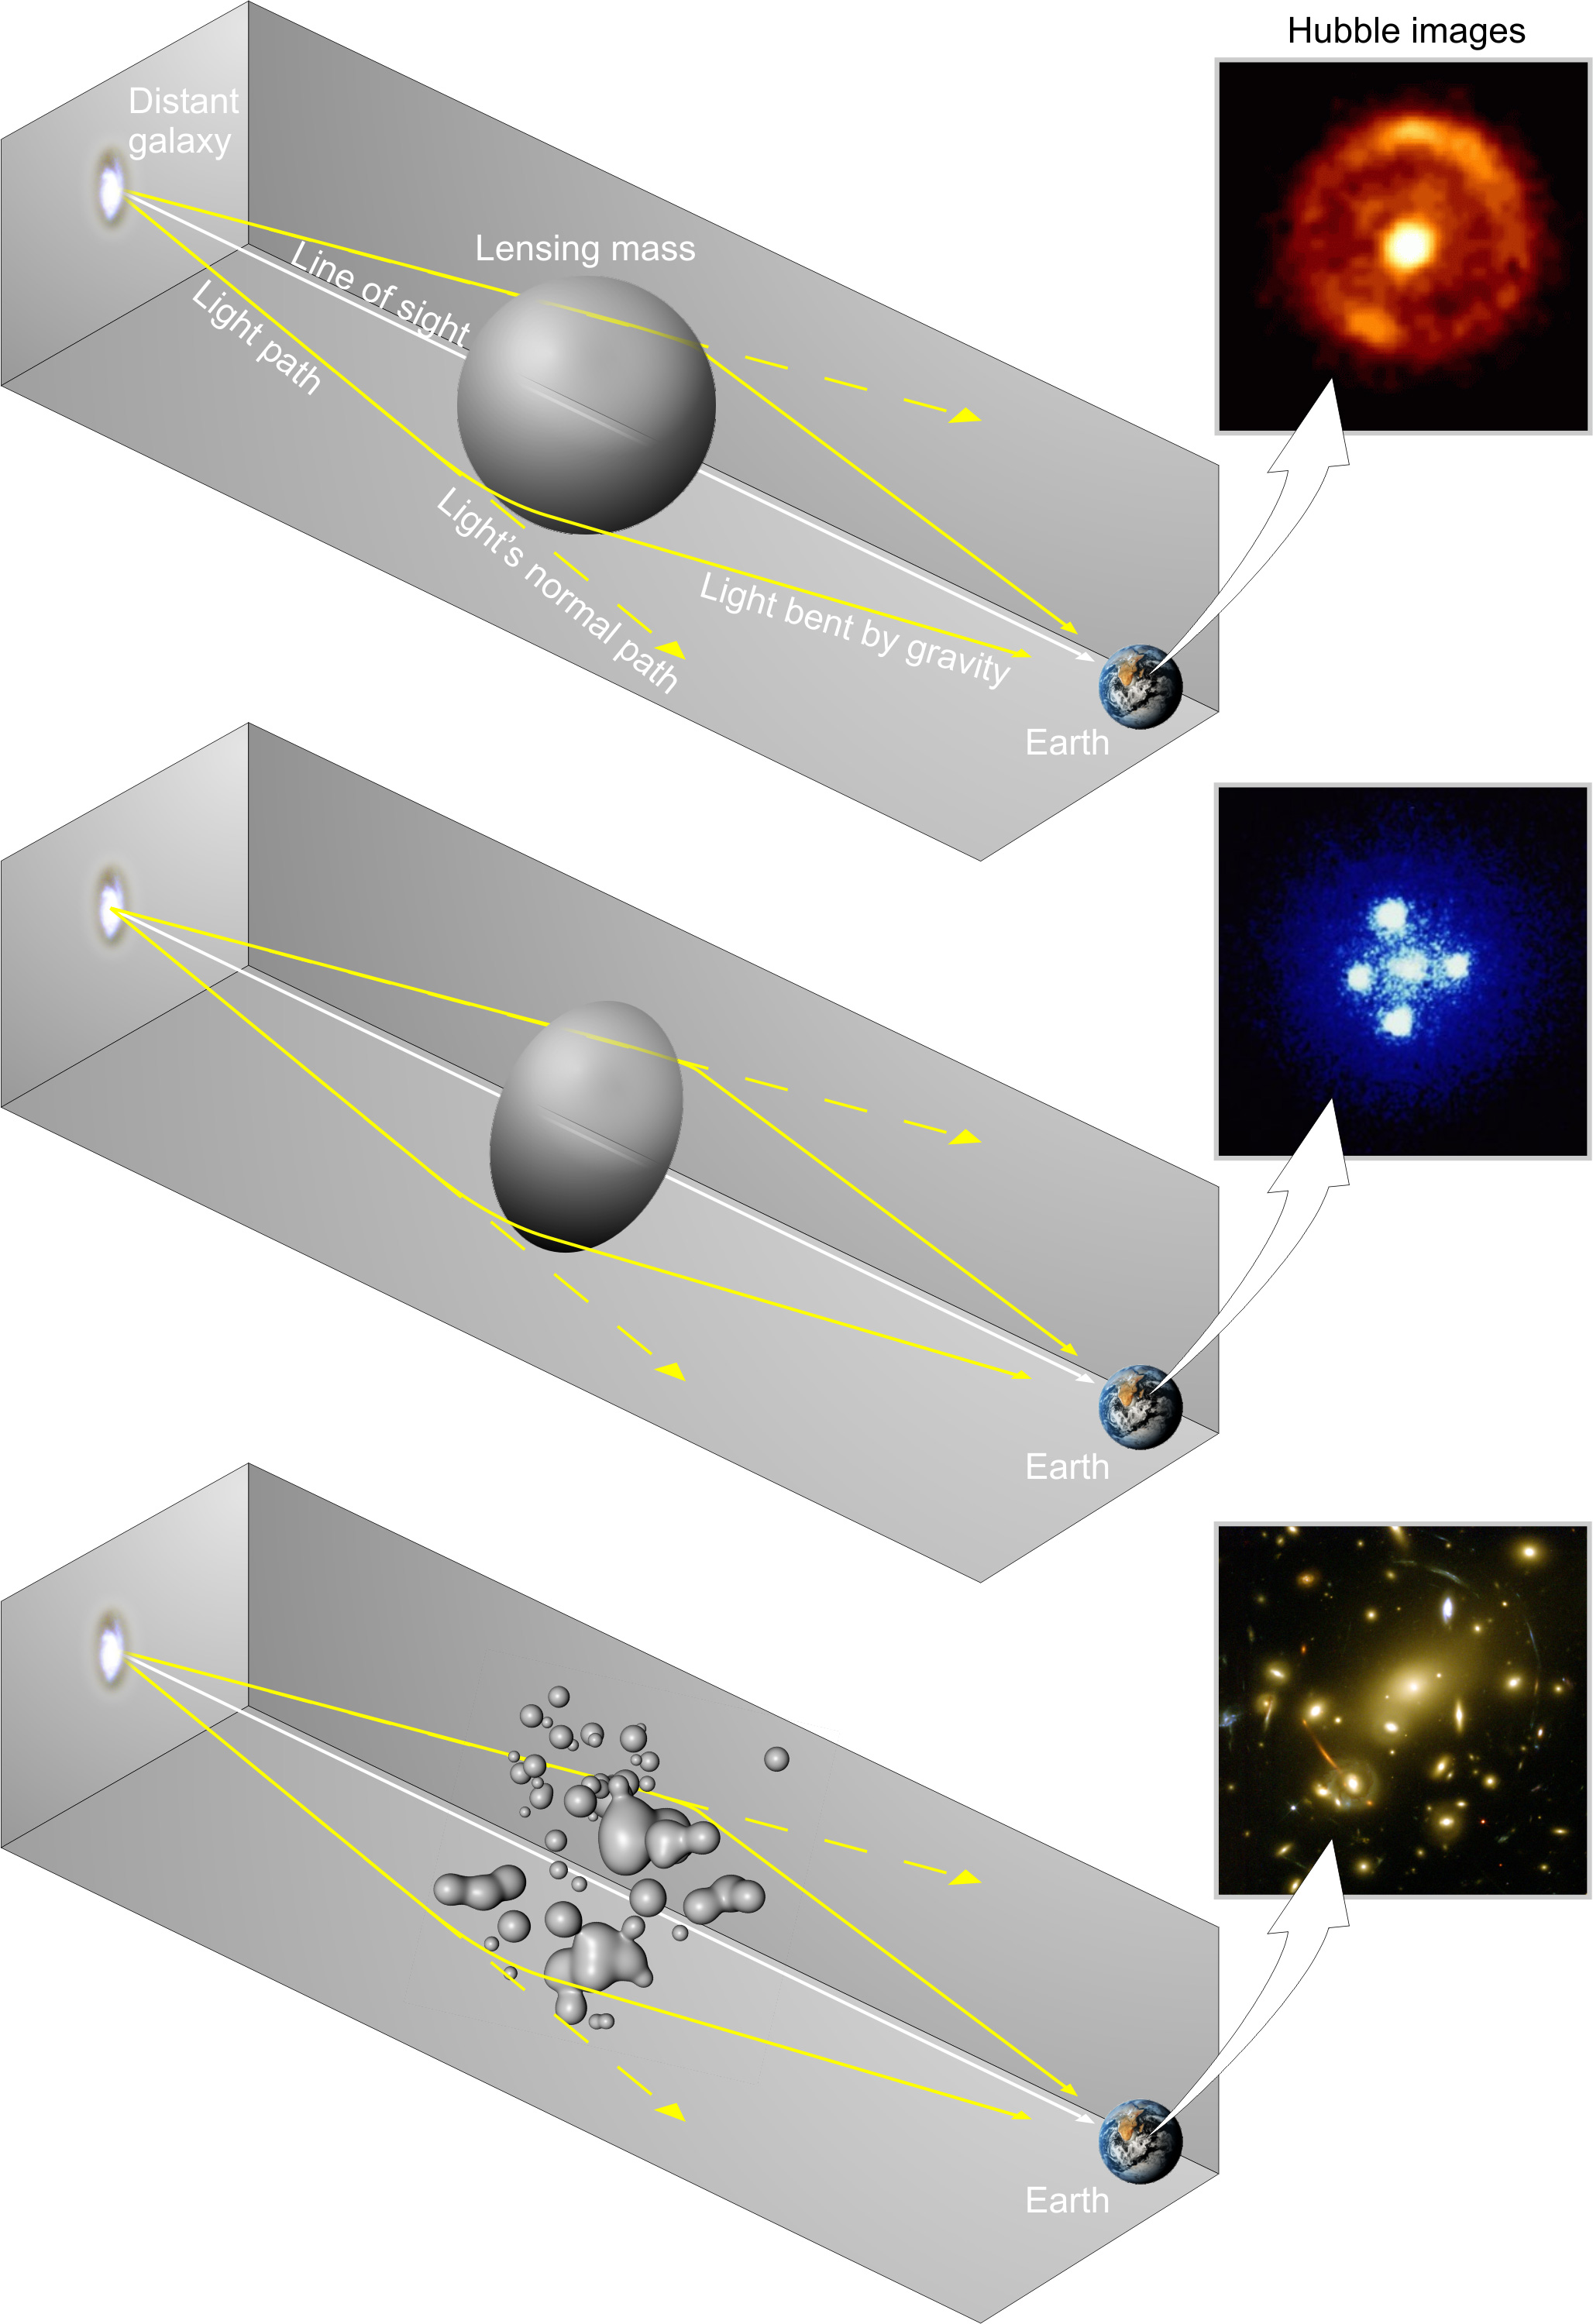
\includegraphics[scale=0.19]{figures/heic0404b.jpg}
        \caption{Light from distant galaxy is bent in different way depending on the distribution of mass between the galaxy and Earth. Yellow dashed lines indicate where the light would have gone if the matter was not present \cite{eas:grav_lensing}.}
        \label{fig:grav_lensing_explained}
    }
\end{figure}

First, micro-lensing observations, or the lack of them, of our Milky Way halo resulted in a conspicuous absence of massive astrophysical compact halo objects (MACHOs).
The hypothesis was that 'dark matter' could be accounted for by sufficiently dim compact objects.
Such objects include things like planets, brown dwarves, black holes, or neutron stars.
Whenever these objects passed in front of a large luminous source, such as the Large Magelenic Clouds, a variation in light should be observed \cite{Hooper:DMHistory}.
The MACHO and EROS collaborations performed this observation and did not find a substantial contribution to the DM Milky Way halo from MACHOs.
They measured that MACHOs of mass range 0.15 to 0.9 $M_{\sun}$ contributes to an upper limit of 8\% of the DM halo mass \cite{Tisserand:MACHO}.

\begin{figure}[ht]
    \centering{
        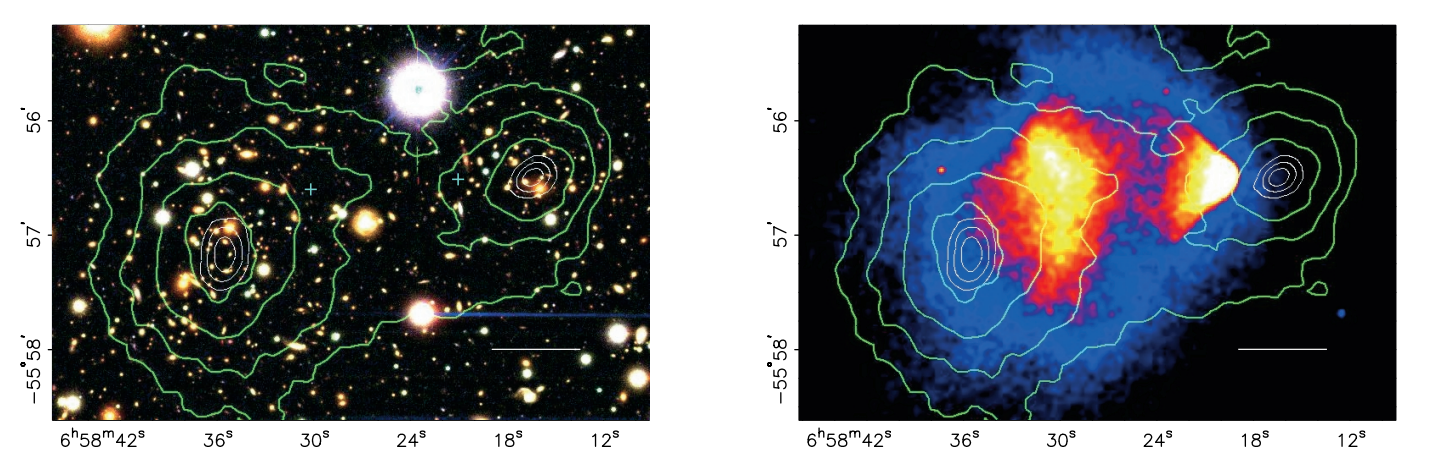
\includegraphics[scale=0.425]{figures/bullet_cluster.png}
        \caption{(left) Optical image of galactic cluster. (right) X-ray image of the cluster with redder meaning hotter and higher baryon density. (both) Green contours are reconstruction of gravity contours from micro-lensing. White rings are the best fit mass maxima at 68.3\%, 95.5\%, and 99.7\% confidence. Maxima of the clusters are clearly separated from x-ray maxima. \cite{Clowe:BulletCluster}}
        \label{fig:bullet_cluster}
    }
\end{figure}

Gravitational lensing can also be applied towards galaxy clusters for DM searches.
The observation of two merging galactic clusters in 2006, shown in \cref{fig:bullet_cluster}, provided a compelling arguement for particle DM outside the Standard Model.
These clusters merged recently in astrophysical time scales.
They're recent merge separated the stars and galaxies are separated from the intergalactic gas.
For these clusters, the hot, intergalactic gas is responsible for most of the mass in the systems \cite{Hooper:DMHistory}.
The hot gas is observed from its x-rays emmision.
Two observations of the clusters were made independantly of each other.
The first was the microlensing of light around the galaxies due to their gravitational influences.
When celestial bodies are large enough, the gravity they exert bends space and time itself.
This bending effects light and will deflect light in a smilar way to how lenses will bend light.
With a sufficient understanding of light sources behind a celestial body, we can reconstruct the countours of the gravitational lenses.
The gradient of the contours then indicates how dense the matter is and where it is.

The x-ray emmision can then be observed from the clusters.
Since these galaxies are mostly gas and are merging, then the gas should be getting hotter.
If they're merging, the x-ray emmisions should be the strongest where the gas is mostly moving through each other.
Hence, X-ray emmision maps out where the gas is in the merging galaxy cluster.

The micro-lensing and x-ray observations were done on the Bullet cluster featured on \cref{fig:bullet_cluster}.
The x-ray emmisions does not align with the gravitational countours from microlensing.
The incongruence in mass density and baryon density suggests that there is a lot of matter somewhere that does not interact with light.
Moreover, this dark matter is can not be baryonic \cite{Clowe:BulletCluster}.
The Bullet Cluster measurement did not really tell us what DM is exactly, but it did give the clue that DM also does not interact with itself very strongly.
If DM did interact strongly with itself, then it would have been more aligned with the x-ray emmision \cite{Clowe:BulletCluster}.
There have been follow-up studies of galaxy clusters with similar results.
The Bullet Cluster and others like it provide a strong case against something possibly amiss in our gravitational theories.

%$$$$$$$$$$$$$$$$$$$$$$$$$$$$$$$$$$$$$$$$$$$$$$$$$$$$$$$$$$$$$$$$$$$$$$$$$$$$$$$$$$$%
\subsection{Evidence for Dark Matter: Cosmic Microwave Background\label{sec:ev4dm_cmb}}
%$$$$$$$$$$$$$$$$$$$$$$$$$$$$$$$$$$$$$$$$$$$$$$$$$$$$$$$$$$$$$$$$$$$$$$$$$$$$$$$$$$$%

\begin{figure}[ht]
    \centering{
        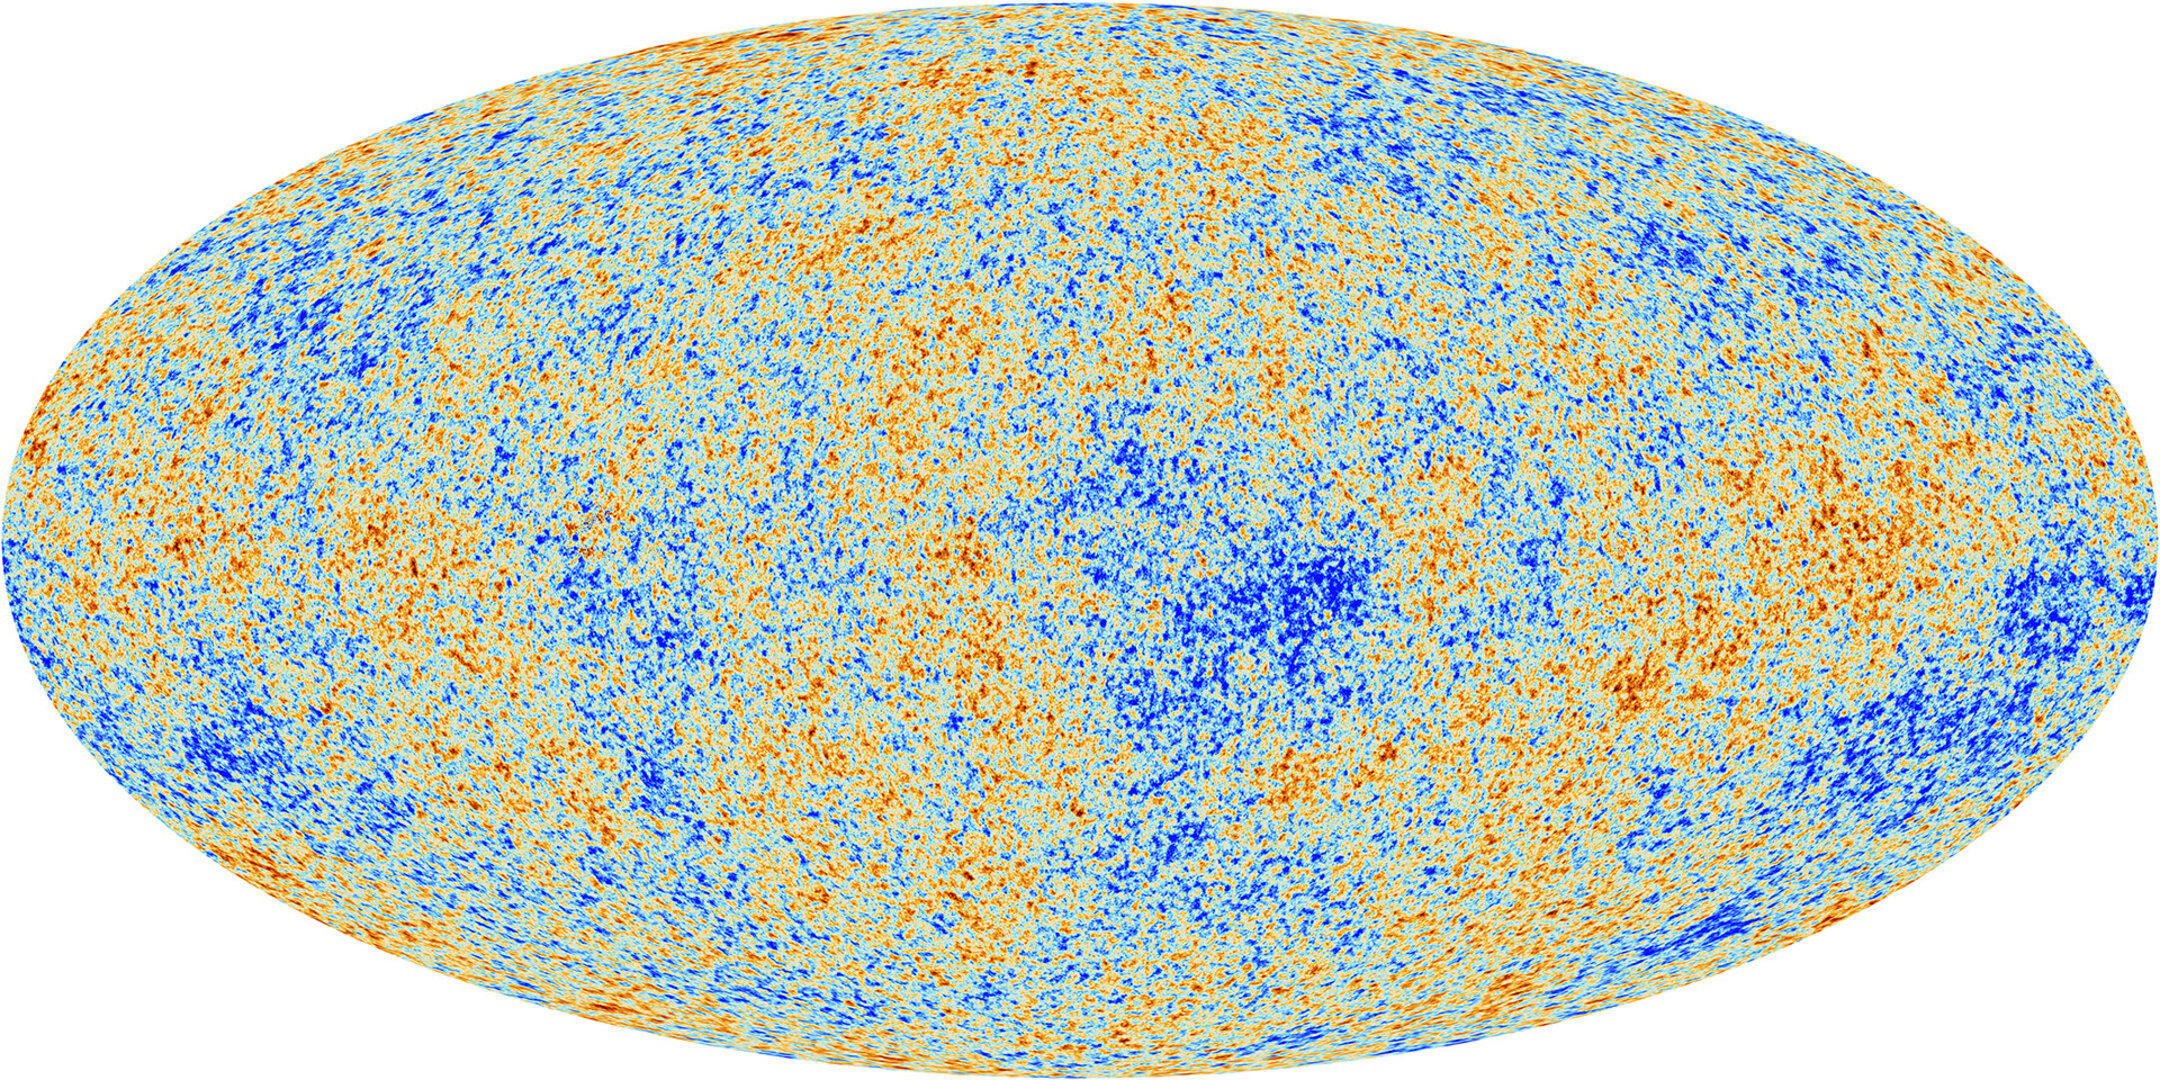
\includegraphics[scale=0.215]{figures/Planck_CMB_pillars.jpg}
        \caption{Plank CMB sky. Sky map features small variations in temperature in primordial light. These anisotropies can be used to make inferences about the universe's energy budget. \cite{Plank:CMB}}
        \label{fig:CMB}
    }
\end{figure}

The Cosmic Microwave Background (CMB) is the primordial light from the early universe when Hydrogen atoms formed from the free electron and proton soup in the early universe.
The CMB is the earliest light we can observe; released when the universe was about 380,000 years old.
Then we look at how the simulated universes look like compared to what we see.
\cref{fig:CMB} is the most recent CMB image from the Plank observatory \cite{Plank:CMB}.
Redder regions indicate a slightly hotter region of the early universe and blue indicates colder.

\begin{figure}[ht]
    \centering{
        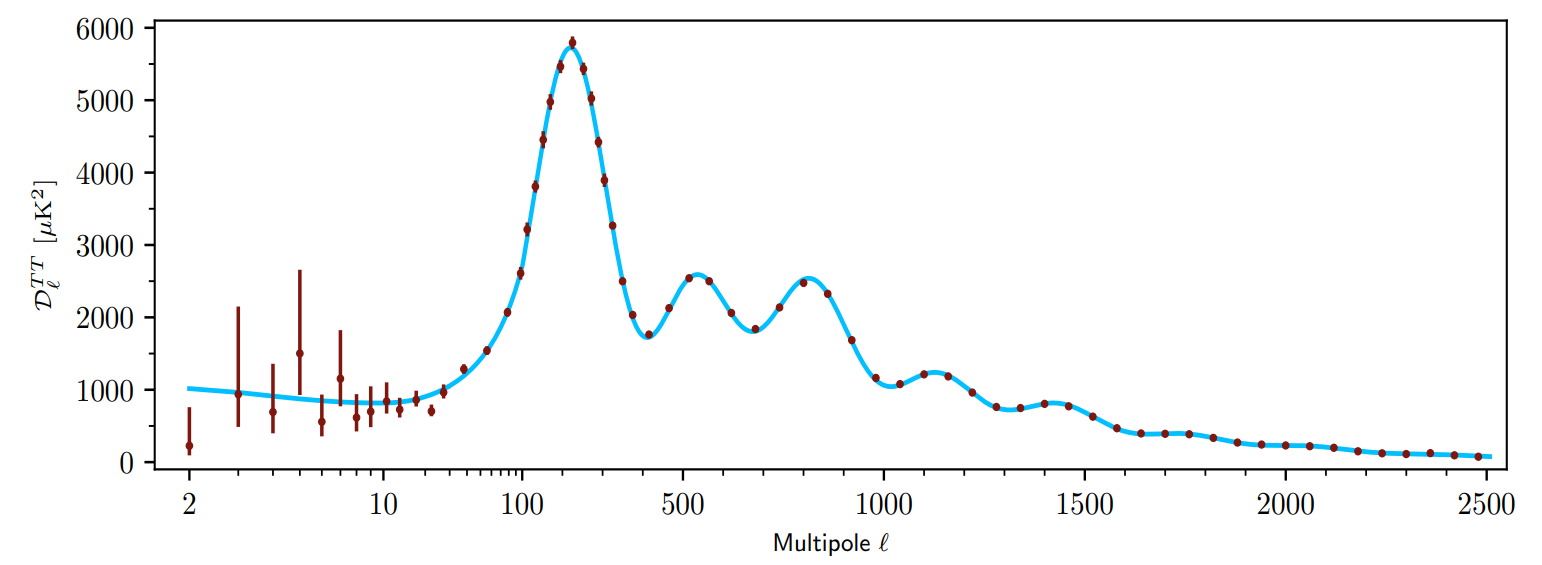
\includegraphics[scale=0.4]{figures/multipole.png}
        \caption{Observed Cosmic Microwave Background power spectrum as a function of multipole momentfrom Plank \cite{Plank:CMB}. Blue line is best fit model from \lcdm. Red points and lines are data and error respectively. }
        \label{fig:multipole}
    }
\end{figure}

To measure the DM, Dark Energy, and matter fractions of the universe from the CMB, the image is deconstructed into a power spectrum versus spherical multipole moments.
\lcdm~provides the best fit to the power spectra of the CDM as shown in \cref{fig:multipole}.
The CMB power spectrum is very senstive to the fraction of each energy contribtion in the early universe.
Low \textit{l} modes are dominated by variations in gravitational potential.
Intermediate \text{l} emerge from oscillations in photon-baryon fluid from competing baryon pressures and gravity.
High \textit{l} is a damped region from the diffusion of photons during electron-proton recombination. \cite{Greene:cosmology_dm}

\begin{figure}[ht]
    \centering{
        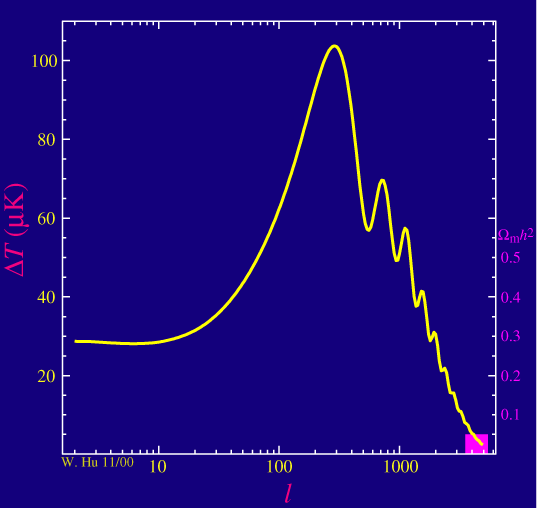
\includegraphics[scale=0.285]{figures/LCDM_multipole/frame_00_delay-0.2s.png}\hfill
        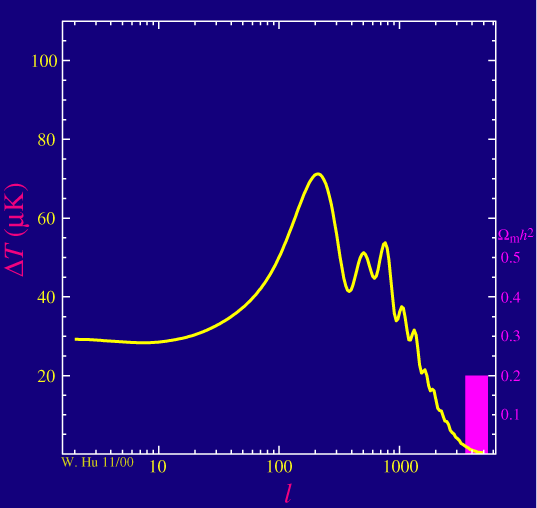
\includegraphics[scale=0.285]{figures/LCDM_multipole/frame_06_delay-0.2s.png}\hfill
        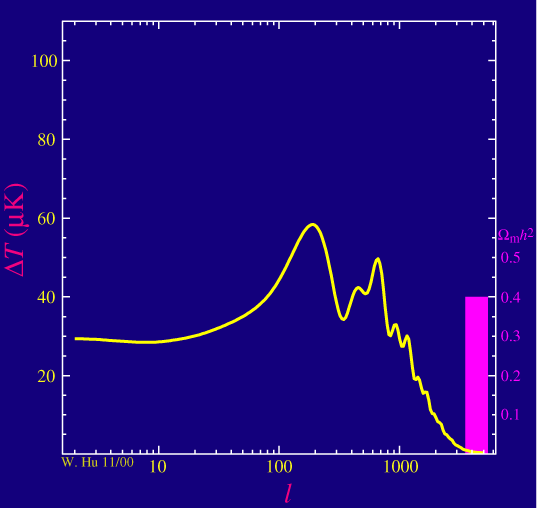
\includegraphics[scale=0.285]{figures/LCDM_multipole/frame_16_delay-0.2s.png}
        \caption{Predicted power spectra of CMB for different $\Omega_m h^2$ values. (left) Low $\Omega_m h^2$ increases the prominence of first and second peaks. (middle) $\Omega_m h^2$ is most similar to the observed power spectrum. The second and third peaks are similar in height. (right) $\Omega_mh^2$ is large which suppresses the first peak and raises the prominence of the third peak.}
        \label{fig:CMB_vibratemodes}
    }
\end{figure}

The harmonics would look very different for a universe with less DM.
\cref{fig:CMB_vibratemodes} shows the differences expected in the power spectrum for different baryon fractions of the universe's energy budget.
The observations fit well with the \lcdm~model and the derived fractions are as follows.
The matter fraction: $\Omega_m = 0.3153$; and the baryon fraction: $\Omega_b = 0.04936$ \cite{Plank:CMB}.
These findings do rely however on a few assumptions and the precision of the Hubble constant, $H_0$.
$H_0$ especially has seen a growing tension in recent decades that continues to deepened with observatories like the James Webb Telescope \cite{JWST:hubble_tension,Freedman:hubble_tension}

Overall these observations form a compelling body of research in favor of dark matter.
However, these observations really only confirm that DM is there.
It takes another leap of theory and experimentation to make observations of DM that are non-gravitational in nature.
One hypothesis is the Weakly Interacting Massive Particle DM.
This DM candidate theory is discussed further in the next section and is the hypothesis to this thesis.

%-----------------------------------------------------------------------------------%
\section{Searching for Dark Matter}\label{sec:dm_search}
%-----------------------------------------------------------------------------------%

There remains many options available to what Dark Matter could be.
For a particle dark matter hypothesis, we asssume that DM interacts in some way, even if very weakly, with the Standard Model (SM), see \cref{fig:SM}.
\begin{figure}[ht]
    \centering{
        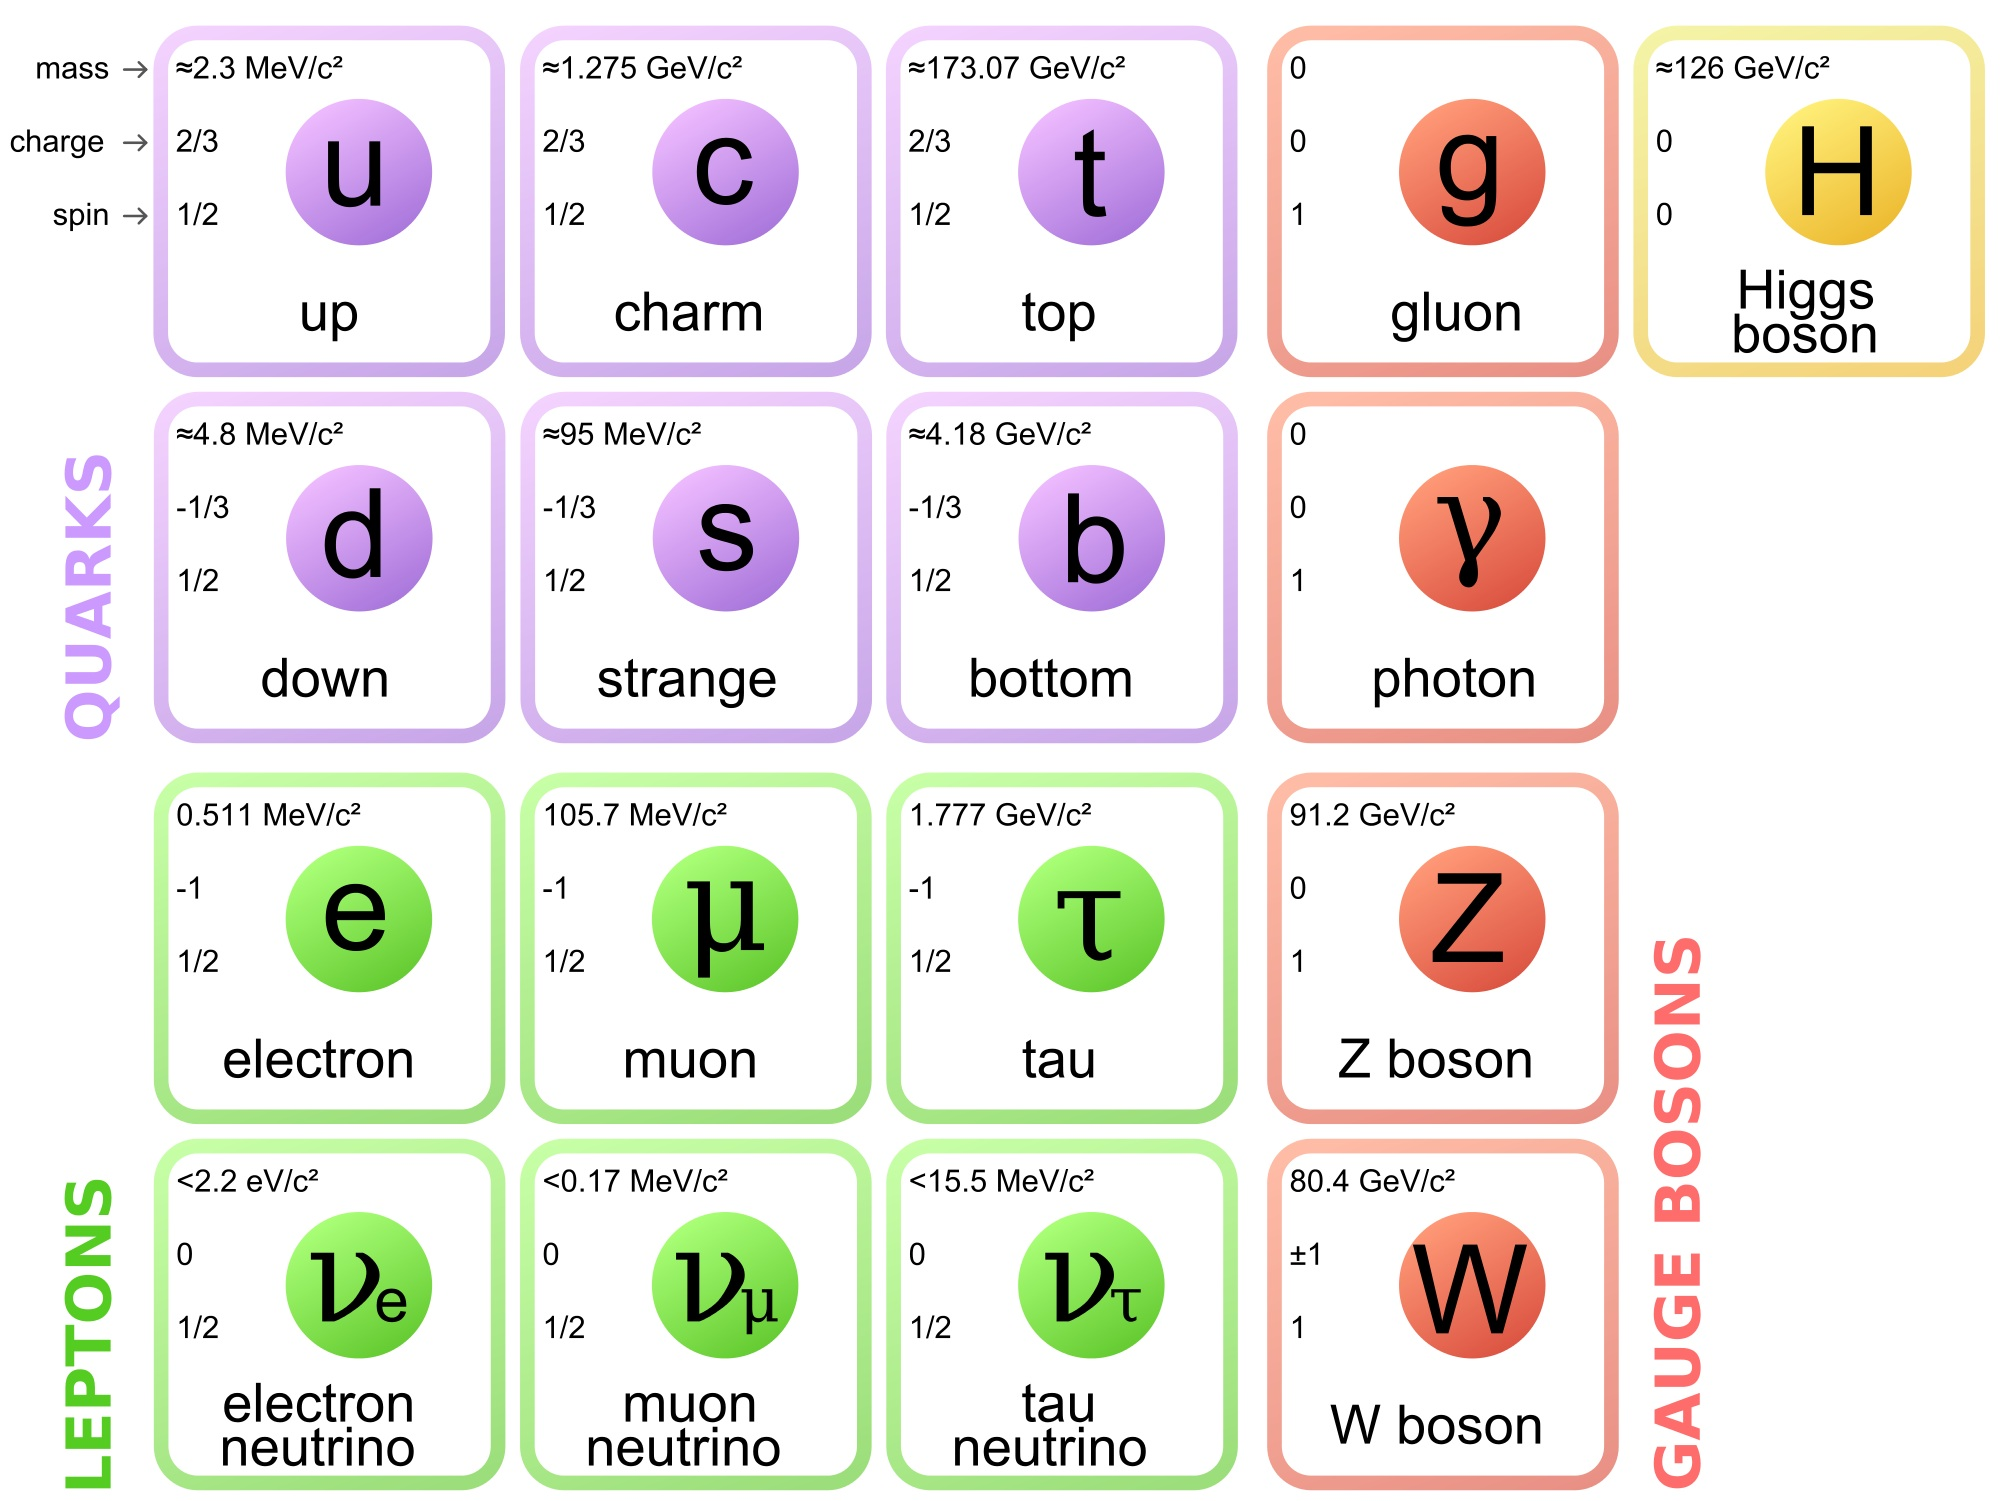
\includegraphics[scale=0.225]{figures/SM.jpg}
        \caption{The Standard Model (SM) of particle physics. Figure taken from \url{http://www.quantumdiaries.org/2014/03/14/the-standard-model-a-beautiful-but-flawed-theory/}}
    }\label{fig:SM}
\end{figure}
The current status of the SM does not have a viable DM candidate.
When looking at the standard model, we can immediately exclude any charged particle.
This is because charged particles interact with light.
If DM is charged, it would be immediately visible if it had similar charge to many SM particles.
Specifically this will rule out the following charged, fundamental particles: $e,\mu, \tau, W, u, d, s, c, t, b$ and their corresponding antiparticles.
Recalling from earlier that DM must be long lived and stable over the age of the universe, this would exclude all SM particles with decay half-lives at or shorter than the age of the universe.
The lifetime constraint additionally eliminates the $Z$ and $H$ bosons.
Finally, the candidate DM needs to be somewhat massive.
Recall from \cref{sec:basicDM} that DM is cold or not relativistic through the universe.
This eliminates the remaining SM particles: $\nu_{e, \mu, \tau}, g, \gamma$ as DM candidates.
Because there are no DM candidates within the SM, the DM problem strongly hints to physics beyond the SM (BSM).


%$$$$$$$$$$$$$$$$$$$$$$$$$$$$$$$$$$$$$$$$$$$$$$$$$$$$$$$$$$$$$$$$$$$$$$$$$$$$$$$$$$$%
\subsection{Shake it, Break it, Make it\label{sec:bop_it}}
%$$$$$$$$$$$$$$$$$$$$$$$$$$$$$$$$$$$$$$$$$$$$$$$$$$$$$$$$$$$$$$$$$$$$$$$$$$$$$$$$$$$%

\begin{figure}[h]
    \centering{
        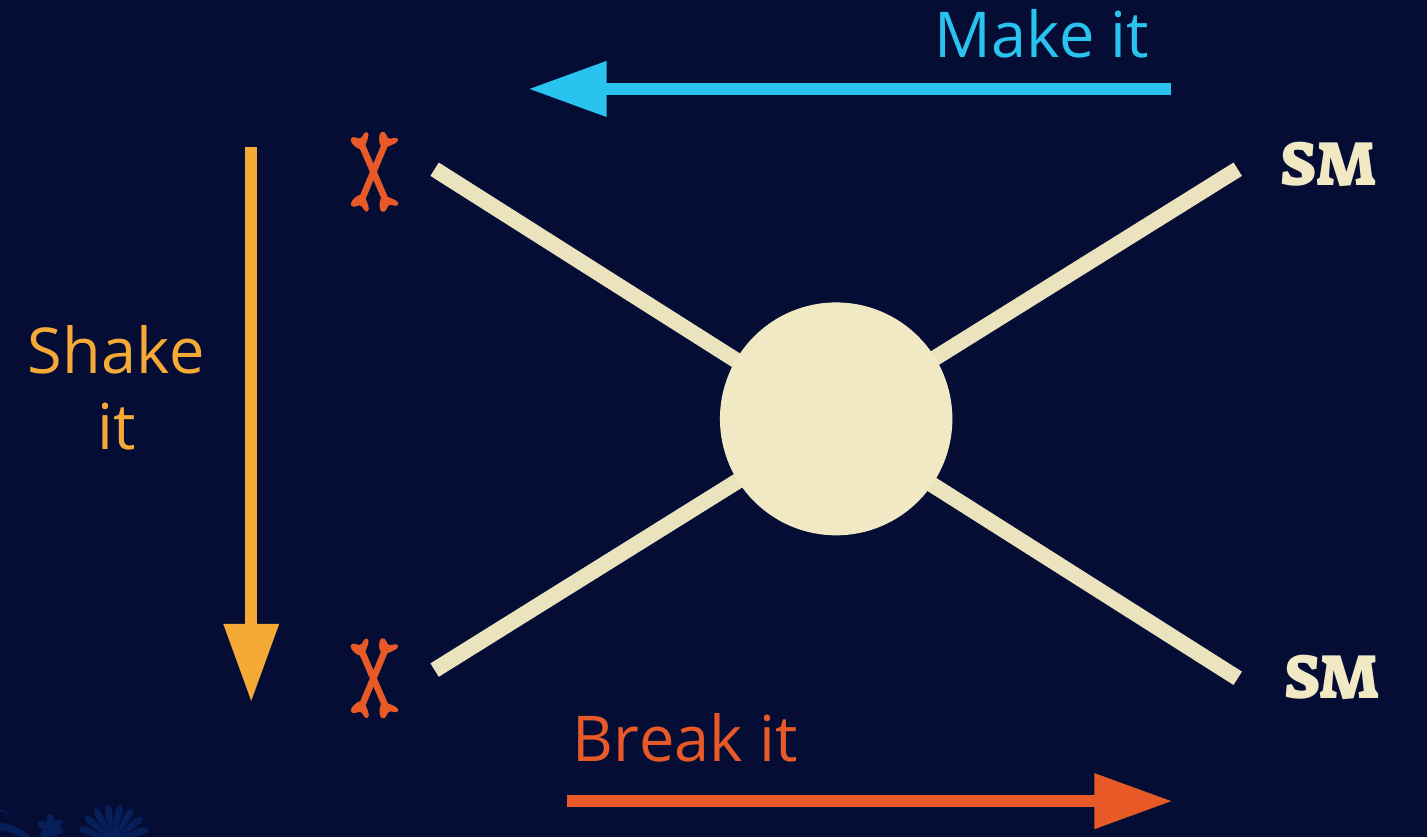
\includegraphics[scale=0.38]{figures/DM_with_SM.png}
        \caption{Simplified Feynman diagram demonstrating with different ways DM can interact with SM particles. The 'X's refer to the DM particles whereas the SM refer to fundamental particles in the SM. The large circle in the center indicates the vertex of interaction and is purposely left vague. The colored arrows refer to different directions of time as well as their respective labels. The arrows indicate the initial and final state of the DM -SM interaction in time.}
        \label{fig:break_it}
    }
\end{figure}

When considering DM that couples in some way with the SM, the interactions are roughly demonstrated by interaction demonstrated in \cref{fig:break_it}.
The figure is a simplified Feynman diagram where the arrow of time represents the interaction modes of: \textbf{Shake it, Break it, Make it}.

\textbf{Shake it} refers to the direct detection of dark matter.
Direct detection interactions start with a free DM particle and some SM particle.
The DM and SM interact under some elastic or inelastic collision and recoil away from each other.
The DM remains in the dark sector and imparts some momentum onto the SM particle.
The hope is that the momentum imparted onto the SM particle is sufficiently high enough to pick up with highly sensitive instruments.
Because we cannot create the DM in the lab, a direct detection experiment must wait until DM is incident on the detector.
Most direct detection experiments are therfore placed in low-background environments with inert detection media like the noble gas Xenon. \cite{Cooley:dd_dm}

\textbf{Make it} refers to the production of DM from SM initial states.
The experiment starts with particles in the SM.
These SM particles are accelerated to incredibly high energies and then collided with each other.
In the confluence of energy, DM hopefully emerges as a byproduct of the SM annihilation.
Often it is the collider experiments that are able to generate energies high enough to probe DM production.
These experiments include the world-wide collaborations ATLAS and CMS at CERN where protons are collided together at extreme energies.
The DM searches however are complex.
DM likely does not interact with the detectors and lives long enough to escape the detection apparati of CERN's colliders.
This means any DM production expirement searches for an excess of events with missing momentum or energy in the events.
An example event with missing transverse momentum is shown in \cref{fig:met_atlas}.
The missing momentum with no particle tracks implies a neutral particle carried the energy out of the detector.
However, there are other neutral particles in the SM, like neutrons or neutrinos, so any analysis have to account for SM signatures of missing momentum. \cite{atlas:met_dm_precise}

\begin{figure}[h]
    \centering{
        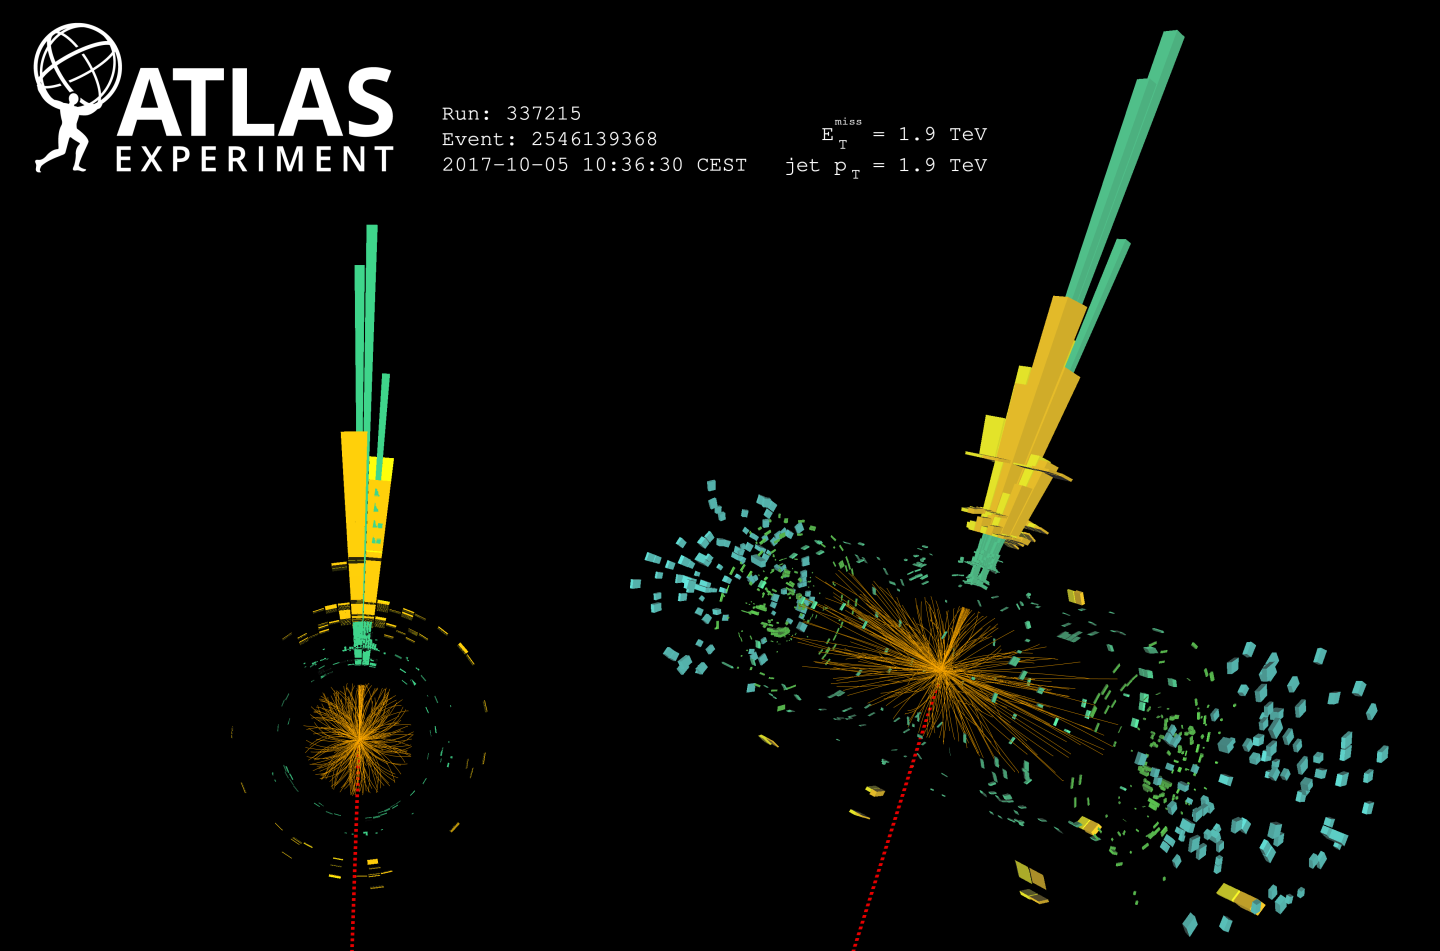
\includegraphics[scale=0.435]{figures/MET_ATLAS.png}
        \caption{A single jet event in ATLAS detector from 2017 \cite{atlas:dm_precise}. Jet momentum observed to be 1.9 TeV. Missing transverse momentum observed to be 1.9 TeV as the initial momentum of the event was 0. Implied MET is shown as a red dashed line in event display.}
        \label{fig:met_atlas}
    }
\end{figure}

%$$$$$$$$$$$$$$$$$$$$$$$$$$$$$$$$$$$$$$$$$$$$$$$$$$$$$$$$$$$$$$$$$$$$$$$$$$$$$$$$$$$%
\subsection{Break it: Standard Model Signatures of Indirect Dark Matter Searches\label{sec:break_it}}
%$$$$$$$$$$$$$$$$$$$$$$$$$$$$$$$$$$$$$$$$$$$$$$$$$$$$$$$$$$$$$$$$$$$$$$$$$$$$$$$$$$$%

\textbf{Break it} refers to the creation of SM particles from the dark sector, and it is the primary focus of this thesis.
The interaction begins with DM or in the dark sector.
The hypothesis is that this DM will either annihilate with itself or decay and produce a SM byproduct.
This method is often refered to the Indirect Detection of DM because we have no lab to directly control or manipulate the DM.
Therefor most DM primary observations will be performed from observations of known DM densities among the astrophysical sources.
The strength is that we have the whole of the universe and it's 13.6 billion year lifespan to use as the detector or particle accelerator.
Additionally, locations of dark matter are also well understood since it was astrophysical observations that presented the problem of DM in the first place.

\begin{figure}[ht]
    \centering{
        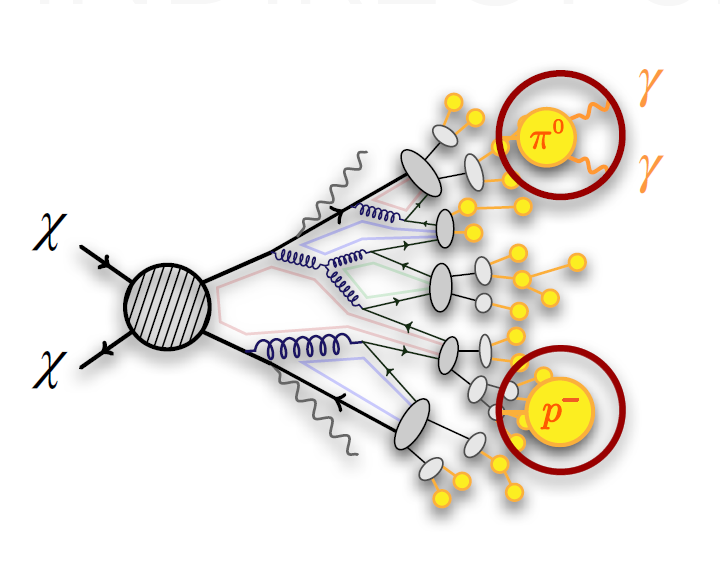
\includegraphics[scale=0.4]{figures/DM_annihilation.png}
        \caption{More detailed pseudo-Feynman diagram of particle cascade from dark matter annihilation into 2 quarks. The quarks hadronize and down to stable particles like \textgamma~or the anti-proton ($p^-$). Diagram pulled from ICRC 2021 presentation on DM annihilation search \cite{2021ICRC:glory_duck}.}
        \label{fig:id_dm_ann}
    }
\end{figure}

However, anything can happen in the universe.
There are many difficult to deconvolve backgrounds when searching for DM.
Once prominant example is the galactic center.
There's a lot of DM there since the Milky Way definitely has a lot of DM.
But any signal coming from there is hard to parse apart from the extreme environment of our supermassive black hole, Sagitatrius A* \cite{Tracy:les_houches}
Despite the challenges, any DM model that yields evidence in the other observation two methods, \textbf{Shake it or Make it} must be corraborated with indirect observations of the known DM sources.
Without corroborating evidence, DM observation in the lab is hard-pressed to demonstrate that it is the model contributing to the DM seen at the universal scale.

In the case of WIMP DM, signals are typically described in terms of primary SM particles produced from a DM decay or annihilation.
The SM initial state particles are then simulated to stable final states such as the $\gamma, \nu, p, \text{or } e$ which can traverse galactic lengths to reach Earth.

\cref{fig:id_dm_ann} shows the quagmire of SM particles that emerges from SM initial states that are not stable \cite{2021ICRC:glory_duck}.
There are many different particles with varying energies that can be produced in such an interaction.
For any arbitrary DM source and stable SM particle, the SM flux from DM annihilating to some neutral particle in the SM, $\phi$, from a region in the sky is described by the following
\iddmannilation
In \cref{eq:id_dm_flux}, $\sv$ is the velocity-weighted annihilation cross-section of DM to the SM.
$m_\chi$ refers to the mass of DM, noted with greek letter $\chi$.
$\frac{dN_{\phi}}{dE_\phi}$ is the N particle flux weighted by the particle energy.
An example is provided in \cref{fig:dm_decay_spectra} for the $\gamma$ final state.
The integrated terms are performed over the solid angle, $d\Omega$, and line of sight, l.o.s.
$\rho$ is the density of DM for a location $(r, \theta')$ in the sky.
The terms left of the '$\times$' are often refered to as the particle physics component.
The terms on the right are refered to as the astrophysical component.
For decaying DM, the equation changes to\dots
\iddmdecay
In \cref{eq:id_dm_decay}, $\tau$ is the decay lifetime of the DM.
Just as in \cref{eq:id_dm_flux}, the left and right terms are the particle physics and the astrophysical components respectively.
The integrated astrophysical component of \cref{eq:id_dm_flux} is often called the J-Factor.
Whereas the integrated astrophysical component of \cref{eq:id_dm_decay} is often called the D-Factor.

\begin{figure}[h]
    \centering{
        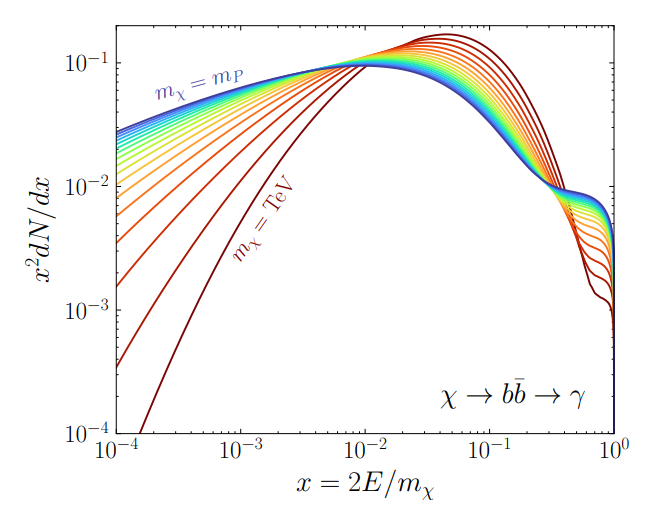
\includegraphics[scale=0.65]{figures/bb_decay_hdm.png}
        \caption{Dark Matter (DM) decay spectrum for $b\bar{b}$ initial state and $\gamma$ final state. Redder spectra are for larger DM masses. Bluer spectra are light DM masses. $x$ is a unitless factor defined as the ratio of the mass of DM, $m_\chi$, and the final state particle energy $E_{\gamma}$. Figure from \cite{Rodd:HDM_spec}.}
        \label{fig:dm_decay_spectra}
    }
\end{figure}

Exact DM DM $\rightarrow$ SM SM branching ratios are not known, so it is usually assumed to go 100\% into a SM particle/anti-particle.
Additionaly, when a DM annihilation or decay produces one of the neutral, long-lived SM particles ($\nu$ or $\gamma$), the particle can be traced back to a DM source.
For DM above GeV energies, there are very few SM processes that can produce particles with such a high energy.
Seeing such a signal would almost certainly be an indication of the presence of dark matter.
The universe forunately provides us with the largest volume and lifetime ever for a particle physics experiment.

%-----------------------------------------------------------------------------------%
\section{Sources for Indirect Dark Matter Searches\label{sec:dm_targets}}
%-----------------------------------------------------------------------------------%

\begin{figure}
    \centering{
        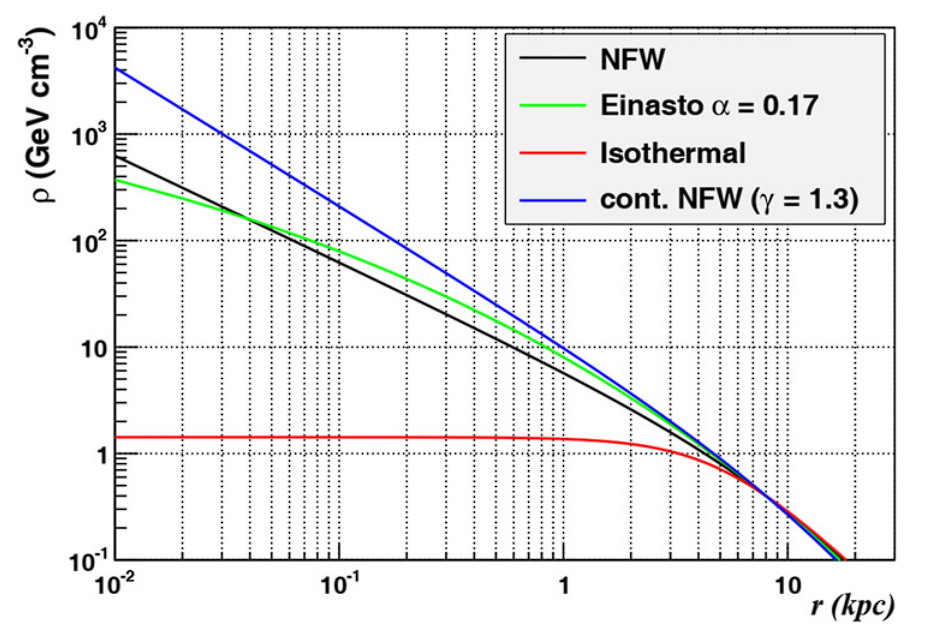
\includegraphics[scale=0.5]{figures/dm_profiles.png}
        \caption{Different dark matter density profiles compared. Some models produce very large densities at small r \cite{2010:dm_profiles}.}
        \label{fig:dm_profile}
    }
\end{figure}

We of course have to know where to look.
Thankfully, we have a good idea of where.
The first detection of DM relied on optical observations.
Since then, we've developed new techniques to find DM dense regions.
As described in \cref{sec:ev4dm_stars}, many DM dense regions were through observing galactic rotation curves.
Our Milky Way galaxy is among DM dense regions discovered, and it is the largest nearby DM dense region to look at.
Additionally, the DM halo surrounding the Milky Way is somewhat clumpy \cite{Tracy:les_houches}.
There are regions in the DM halo of the Milky Way that have more DM than others they have captured gas over time.
In some cases these sub-haloes were dense enough to host stars.
These apparent sub galaxies are known was dwarf spheroidal galaxies and are the main sources studied in this thesis.
Each source type comes with different trade offs.
Galactic Center studies will be very sensitive to the assume distribution of DM.
The central DM density can very substantially as demonstrated in \cref{fig:dm_profile}.
At small r, the differences in DM densities can be 3-4 orders of magnitude.

Dwarf Spheroidal Galaxies (dSph's) studies suffer from uncertainties in the DM density less than the galactic center studies.
This is mostly from their diminutive size being smaller than the angular resolution of most $\gamma$-ray observatories \cite{Tracy:les_houches}.
The DM content dSph's are typically determined with the virial theorem, \cref{eq:virialtheorem}, and are usually majority DM \cite{Tracy:les_houches} in mass.
DSph's tend to be ideal sources to look at for DM searches.
Their environments are fairly quiet with little astrophysical backgrounds.
Unlike the galactic center, the most active components of dSph's are the stars within them versus a violent accretion disc around a black hole.
All this together means that dSph's are among the best sources to look at for indirect DM searches.
dSph's are the targets of focus for this thesis.

%-----------------------------------------------------------------------------------%
\section{Multi-Messenger Dark Matter \label{sec:mult-messengerDM}}
%-----------------------------------------------------------------------------------%

Astrophysics entered a new phase in the past few decades that leverages our increasing sensitivity to SM channels and general relativity (GR).
Up until the 21st century, astrophysical observatations were done with photons ($\gamma$) only.
Astrophysics with this 'messenger' is fairly mature now.
Novel observations of the universe have since only adjusted the sensitivity of the wavelength of light that's observed.
Gems like the CMB \cite{Plank:CMB}, and more have ultimately been observations of different wavelengths of light.
Multi-messenger astrophysics proposes using other SM particles such the $p^{+/-},\text{or } \nu$ or gravitation waves predicted by general relativity.

The expirements LIGO had a revolutionary discovery in 2016 with the first detection of a binary black hole merger \cite{2016:grav_waves}.
This opened the collective imagination entirely to observing the universe through gravitational waves.
There's also been a surge of interest in the neutrino ($\nu$) sector.
IceCube demonstrated that we are sensitive to neutrinos in regions that correlate with significant photon emmission like the galactic plane \cite{2023:IC3_galactic_plane}.
Neutrinos, like gravitational waves and light, travel mostly unimpeded from their source to our observatories.
This makes pointing to the oringinating source of the these messengers much easier than it is for cosmic rays that are almost always deflected from their source.

\begin{figure}[h]
    \centering{
        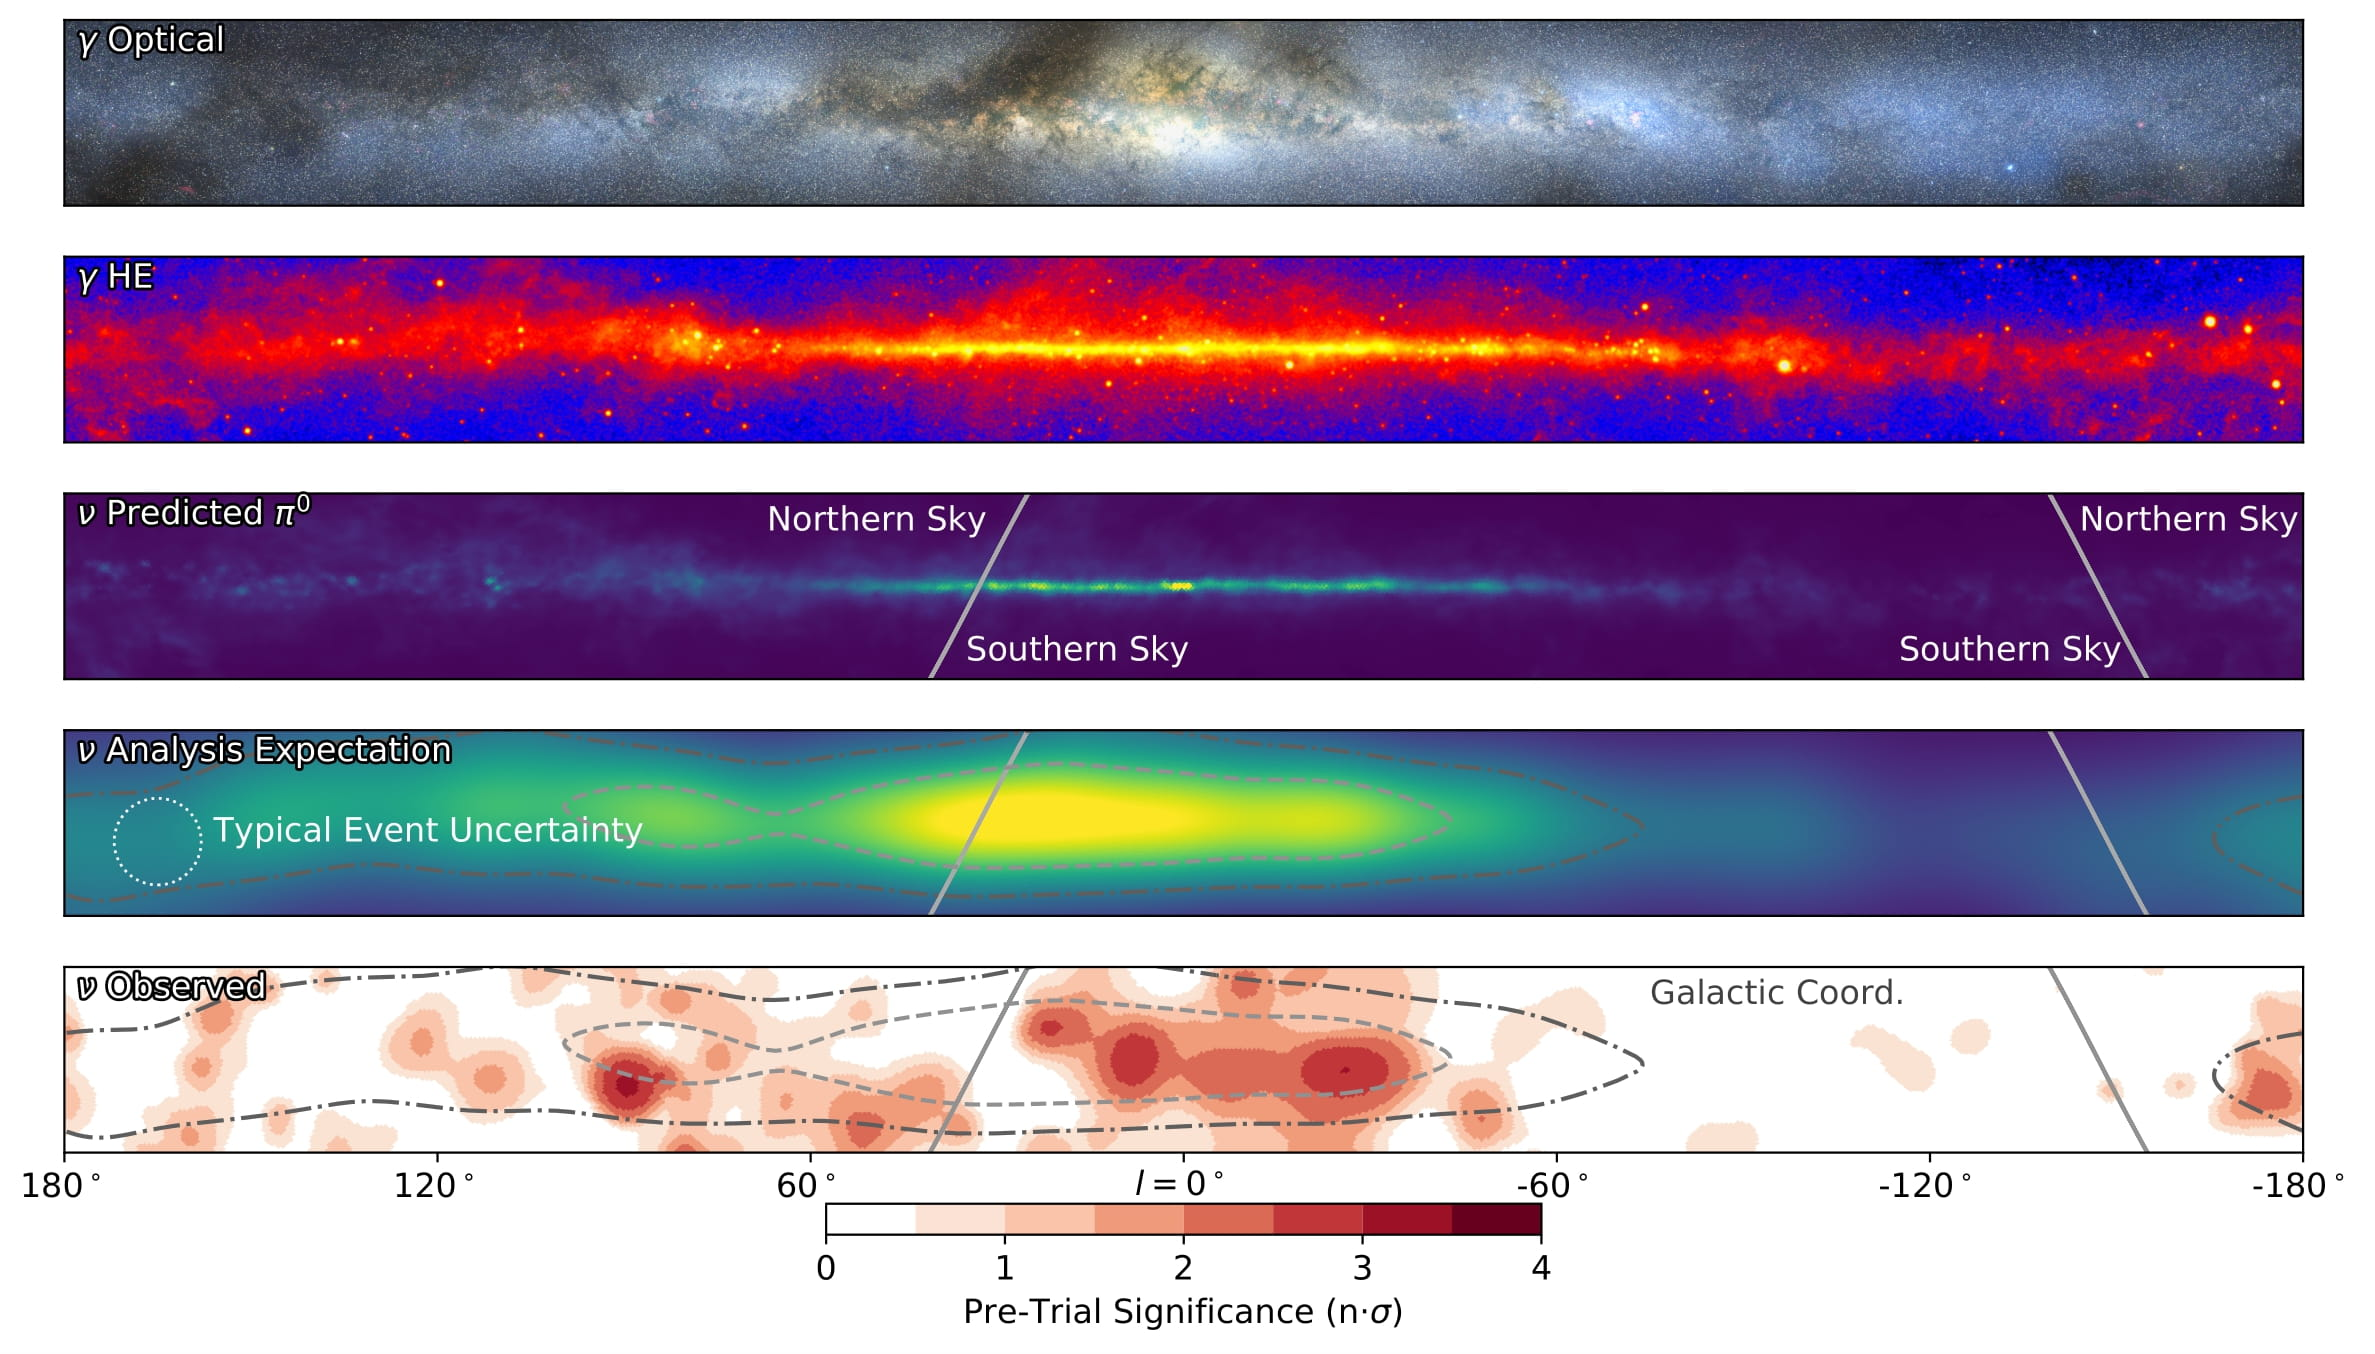
\includegraphics[scale=0.41]{figures/ic3_galacticplane.jpg}
        \caption{The Milky Way Galaxy in photons ($\gamma$) and neutrinos ($\nu$) \cite{2023:IC3_galactic_plane}. Galactic center is at l=0\textdegree and is the brightest region in all panels. (top) An Optical color image of the Milky Way galaxy seen from Earth. Clouds of gas and dust obscure some of the light from stars. (2nd down) Integrated flux of $\gamma$-rays observed by the Fermi-LAT telescope \cite{fermi:mw_plane}. (middle) Expected neutrino emmision that corresponds with Fermi-LAT observations. (2nd up) Expected neutrino emmision profile after considering detector systematics of IceCube. (bottom) Observed neutrino emmision from region of the galactic plane. Substantial neutrino emmision is detected.}
        \label{fig:ic3_mw}
    }
\end{figure}

The recent result from IceCube, shown in \cref{fig:ic3_mw}, proves that we can make obervations under different messenger regimes.
The top two panels are the appearance of the galactic plane to different wavelengths of light.
Some sources are more apparent in some panels, while others are not.
The IceCube collaboration recently published a groundbreaking result of the Milky Way in neutrinos.
This new channel is potential very powerful because neutrinos are readily able to penetrate see through gas and dust in the Milky Way.
This new image also refines our understanding of how high energy particles are accelerated since the fit to IceCube data prefers one standard model process over the other \cite{2023:IC3_galactic_plane}.

\begin{figure}[h]
    \centering{
        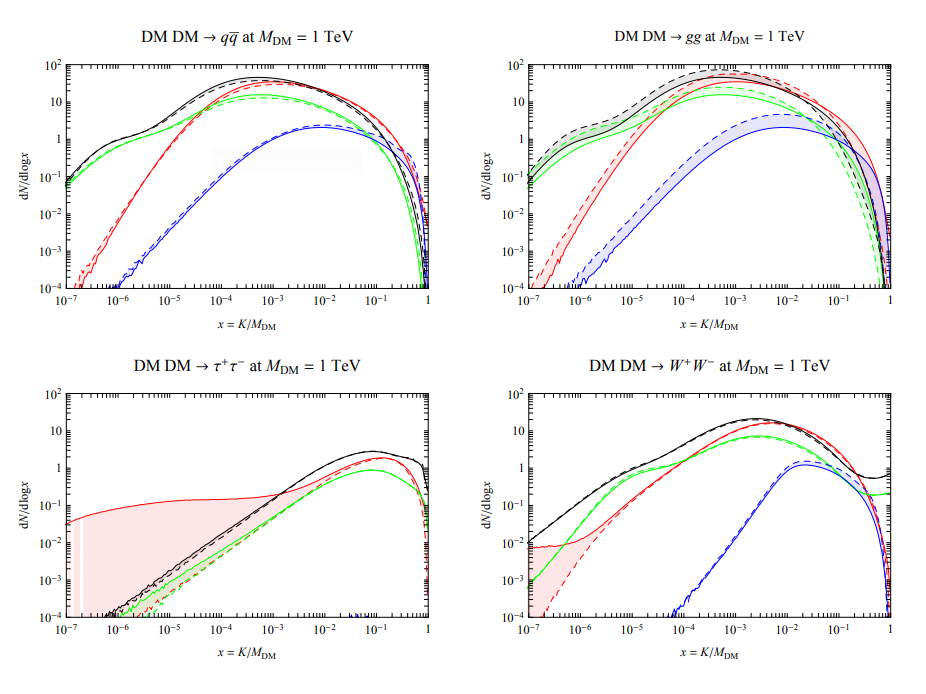
\includegraphics[scale=0.65]{figures/pppc_spectra.png}
        \caption{Dark Matter annihilation spectra for different final state particle and standard model annihilation channels \cite{pppc}. Photons (red), $e^\pm$ (green), $\bar{p}$ (blue), $\nu$ (black).}
        \label{fig:pppc_spectra}
    }
\end{figure}

Exposing our observations to more cosmic messengers greatly increases our sensitivity to rare processes.
In the case of DM, \cref{fig:pppc_spectra},  there are many SM particles produced in a dark matter annihilation.
Among the final state fluxes are gammas and neutrinos.
Charged particles are also produced however they would not likely make it to Earth since they will be deflected by magnetic fields between the source and Earth.
This means observatories that can see the neutral messengers are especially good for DM searches and for combining data for a multi-messenger DM search.
